% TFG - José Ángel Martín Baos. Escuela Superior de Informática. 2018
%%%% CHAPTER: Results %%%
\chapter{Results} % TODO
\label{chap:results}

\drop{I}{n} this chapter, the different results obtained during the execution of this \ac{BSc.} thesis are presented. The working methodology presented in Chapter \ref{chap:methodology} is going to be used to carry out the work. In first place, the initial Sprint is presented, where the Scrum team will be set up, as well as the initial planning of the project. Subsequently, the different Sprints are presented, where the work planned in the initial Sprint will be carried out.




%%% Sprint 0
\section{Sprint 0: Initial planning}
\label{Section:Sprint0}
In this first phase, Sprint 0, the main objective is to define the Scrum team, the user stories, the project plan, and the temporal and cost planning. Then, the draft (“Anteproyecto”) must be written. Once this Sprint has been completed, the project can start, as state in the temporal planning. The task associated to this initial Sprint can be shown in Table \ref{tab:Sprint0-Tasks}.

\begin{table}[hp]
	\centering
	{\small
		\begin{tabular}{|p{.7\textwidth}P{.1\textwidth}|}
	\hline
	\rowcolor{tabheadbg}
	\multicolumn{2}{|c|}{\textscale{.8}{\textbf{Sprint 0 tasks}}} \\
	\hline
	\hline
	\textscale{.8}{\textbf{Task}} 			& \textscale{.8}{\textbf{Estimate}} \\
	\hline
	Define the Scrum team					& 0,5h \\
	\hline
	Define the user stories					& 5h \\
	\hline
	Generate the project plan				& 2h \\
	\hline
	Generate the temporal planning			& 2h \\
	\hline
	Generate the cost planning				& 1h \\
	\hline
	Investigate about similar proposals								& 3h \\
	\hline
	Create a GitHub repository				& 0,5h \\
	\hline
	Write the draft (“Anteproyecto”)		& 21h \\
	\hline
	\textbf{Total} 							& 35h \\
	\hline

\end{tabular}
	}
	\caption{Sprint 0 tasks}
	\label{tab:Sprint0-Tasks}
\end{table}

\subsection{Scrum Team}
Following the scrum roles defined in Section \ref{5-ScrumTeam}, the Scrum team will have the following structure:
\begin{itemize}
	\item \textbf{Product Owner:} Ricardo García Ródenas
	\item \textbf{Scrum Master:} Luis Rodríguez Benítez
	\item \textbf{Development Team:} José Ángel Martín Baos
\end{itemize}

\subsection{Product Backlog}
\REDNOTE{... \& User Stories Table}
\begin{table}[hp]
	\centering
	{\small
		\begin{tabular}{ |P{.08\textwidth}p{.56\textwidth}P{.1\textwidth}P{.14\textwidth}|}
	\hline
	\rowcolor{tabheadbg}
	\multicolumn{4}{|c|}{\textscale{.8}{\textbf{User stories}}} \\
	\hline
	\textscale{.8}{\textbf{ID}}	& \textscale{.8}{\textbf{User history}}	& \textscale{.8}{\textbf{Priority}}	& \textscale{.8}{\textbf{Estimation (h)}} \\
	\hline
	1 	& Configure Raspberry Pi Architecture 										& High 		& 15 \\ 
	\hline
	2 	& Install PiCamera module in the Raspberry Pi								& High 		& 5 \\ 
	\hline	
	3 	& Develop an algorithm to calculate the vehicle flow		 				& High 		& 30 \\ 
	\hline
	4 	& Install environmental and gas sensors into Raspberry Pi					& High 		& 25 \\ 
	\hline
	5 	& Obtain and process data from the sensors									& High 		& 30 \\ 
	\hline
	6 	& Develop a comunication module using IBM IoT								& High 		& 15 \\ 
	\hline
	7 	& Receive sensor data from the Raspberry Pi and store it into a Database	& High 		& 12 \\ 
	\hline
	8 	& Integrate camera, sensors and comunication module into an unique program	& Medium	& 8 \\ 
	\hline
	9 	& Design a web page to monitor the data obtained by the Raspberry Pi devices	& High 		& 10 \\ 
	\hline
	10 	& Monitor in real time the data obtained by the devices and send an alert if the pollutant gases exceed a threshold																		& Medium 		& 20 \\ 
	\hline
	11 	& Display the historical data generated by the Raspberry Pi devices			& Low	& 20 \\ 
	\hline	

\end{tabular}
	}
	\caption{User stories}
	\label{tab:User-Stories}
\end{table}
	
The different user stories are presented its corresponding Sprints. Each user story is formed by the following fields:
\begin{itemize}
	\item \emlst{Sprint.} It indicates the Sprint number to which the user story belongs to.
	\item \emlst{Priority.} Priority given to the user story. It can take the values: low, medium and high.
	\item \emlst{Effort.} The estimated duration of the user story in hours. 
	\item \emlst{Name.} The label of the user story.
	\item \emlst{Description.} It is a brief definition of the user story.
	\item \emlst{Tasks.} It consists in a list of the different tasks that must be executed to complete the user story.
	\item \emlst{Tests.} It is a list of the different tests defined for the user story.
\end{itemize}

\subsection{Project plan}
\REDNOTE{Different sprints and its associated user stories and time estimation. \\
What is the total duration of the \ac{BSc.} Thesis?}
\begin{table}[hp]
	\centering
	{\small
		\begin{tabular}{|P{.08\textwidth}p{.56\textwidth}P{.15\textwidth}P{.08\textwidth}|}
	\hline
	\rowcolor{tabheadbg}
	\multicolumn{4}{|c|}{\textscale{.8}{\textbf{Sprints}}} \\
	\hline
	\hline
	\textscale{.8}{\textbf{Sprint}}			& \textscale{.8}{\textbf{Name}}	& \textscale{.8}{\textbf{User stories}}	& \textscale{.8}{\textbf{Estimate}} \\
	\hline
	0 	& Initial planning		 	& - 	& 35h \\ 
	\hline
	1 	& Development a basic algorithm to calculate the flow of vehicles		 		 	& 1, 2, 3 	& 50h \\ 
	\hline
	2 	& Design of an environmental parameters monitoring system		 	& \REDNOTE{...} 	& \REDNOTE{X}h \\ 
	\hline

\end{tabular}
	}
	\caption{Sprints}
	\label{tab:Sprints}
\end{table}

\subsection{Temporal planning}
\REDNOTE{Using the project plan, translate it to a graph (Remember the “Anteproyecto”)}

\REDNOTE{ Check the duration of all the task and sprints.} %TODO: Check the duration of all the task and sprints

\REDNOTE{The project start in September}

% Ganttproject


\subsection{Cost planning}
To manage the costs for the development of this project, two tables has been elaborated. Table \ref{tab:Hardware-Costs} indicates the costs related with the hardware resources that must be purchase in order to execute the project. Moreover, some development cost must be taken into account, which are indicated in Table \ref{tab:Development-Costs}. For the purpose of calculating the salary of the developer, the \ac{UCLM} retributions table of labor contracts for research projects on 2017 has been used. Therefore, it has been considered that the developer will have “Tercera-O-II” category, meaning that its annual cost will be of $23.598,83$\euro{}

\begin{table}[hp]
	\centering
	{\small
		\begin{tabular}{ |p{.5\textwidth}P{.1\textwidth}r|}
	\hline
	\rowcolor{tabheadbg}
	\multicolumn{3}{|c|}{\textscale{.8}{\textbf{Hardware costs}}} \\
	\hline
	\hline
	\textscale{.8}{\textbf{Item}}	& \textscale{.8}{\textbf{Quantity}}	& \textscale{.8}{\textbf{Cost}} \\
	\hline
	Raspberry Pi 3 					& 2 	& 49\euro{} \\ 
	\hline
	Pi NoIR Camera V2 				& 2 	& 28\euro{} \\ 
	\hline
	Memory card Samsung SDHC
	EVO 8gb Class 10+ 				& 2		& 8\euro{} \\ 
	\hline
	Power bank battery 				& 2 	& 29\euro{} \\ 
	\hline
	Camera Case		 				& 2 	& 14\euro{} \\ 
	\hline
	Raspberry Pi Sense HAT			& 2 	& 42\euro{} \\ 
	\hline
	Stacking Header 40 PIN 			& 2 	& 7\euro{} \\ 
	\hline
	MQ7 Gas Sensor		 			& 2 	& 2.5\euro{} \\ 
	\hline
	MQ2 Gas Sensor 					& 2 	& 3\euro{} \\ 
	\hline
	MCP3008 AD Conversor			& 2 	& 9\euro{} \\ 
	\hline
	Prototype shield  				& 1 	& 1.5\euro{} \\ 
	\hline
	Wires 							& 1 	& 7\euro{} \\ 
	\hline
	LM317 							& 2 	& 1.75\euro{} \\ 
	
	\Xhline{2\arrayrulewidth}
	\textbf{TOTAL:} &  		& \textbf{395\euro{}} \\ 
	\hline

\end{tabular}

	}
	\caption{Hardware costs}
	\label{tab:Hardware-Costs}
\end{table}

\begin{table}[hp]
	\centering
	{\small
		\begin{tabular}{ |p{.1\textwidth}P{.1\textwidth}r|}
	\hline
	\rowcolor{tabheadbg}
	\multicolumn{3}{|c|}{\textscale{.8}{\textbf{Development costs}}} \\
	\hline
	\hline
	\textscale{.8}{\textbf{Sprint}}	& \textscale{.8}{\textbf{Hours}}	& \textscale{.8}{\textbf{Cost}} \\
	\hline
	0			& 35h 			& \REDNOTE{X}\euro{} \\ 
	\hline
	\REDNOTE{XXX}	& \REDNOTE{X}h 		& \REDNOTE{X}\euro{} \\ 
	
	
	\Xhline{2\arrayrulewidth}
	\textbf{TOTAL:} & \textbf{\REDNOTE{X}h} 		& \textbf{\REDNOTE{X}\euro{}} \\ 
	\hline
	
	% Coste: Regla de 3:
	%    12 meses  ---- 23.598,83 euros
	%    X  meses  ---- Y euros
	% Jornada completa: 35 horas semanales

\end{tabular}
	}
	\caption{Development costs}
	\label{tab:Development-Costs}
\end{table}



%%% Sprint 1
\section{Sprint 1: Development a basic algorithm to calculate the traffic flows based on video data}
\label{Section:Sprint1}
According to the project plan, in this sprint, a basic algorithm to calculate the vehicle flow must be developed. This involves executing the task associated to the user stories 1, 2 and 3. This iteration aims to obtain a basic algorithm to count the number of cars that cross a street in a certain amount of time so as to obtain the vehicle flow. \REDNOTE{Then in Sprint X, it will be improved.} To be able to count the number of cars using the PiCamera, \emword{motion vectors} are used. Therefore, a study about this concept has been done before implementing the algorithm. But first, it is necessary to configure the Raspberry Pi architecture and to install the PiCamera. 

\subsection{Sprint planning meeting}
During the planning meeting, the different user stories addressed in this sprint has been analysed. Consequently, they have been divided into several tasks and tests. The three user stories are shown in Tables from \ref{tab:Sprint1-User-story-1} to \ref{tab:Sprint1-User-story-3}.

\UserStoryTable{1}{1}{High}{15}
{Configure Raspberry Pi Architecture}
{The \ac{OS} and all the components must be installed and configured.}
{	\item Install and configure Raspbian \ac{OS}
	\item Install the necessary libraries
}{	\item Check if the system works correctly using SSH connection
	\item Check if python works
}

\UserStoryTable{2}{1}{High}{5}
{Install PiCamera into Raspberry Pi}
{The PiCamera module must be working and some sample videos should be recorded in order to check the camera.}
{	\item Install the PiCamera module
	\item Develop a program to record videos
}{	\item Check if the camera is working correctly
}

\UserStoryTable{3}{1}{High}{30}
{Develop a basic algorithm to calculate the vehicle flow}
{Development of a basic algorithm that counts the number of cars that go across a street and determines their direction.}
{	\item Study the functionality of the motion vectors in H264/AVC
	\item Extract the motion vectors when recording a video with the PiCamera module using PiMotionAnalysis
	\item Read and process the data stored containing the motion vectors
	\item Develop a noise filter using moving averages
	\item Develop the basic algorithm to counts the cars
}{	\item Check the correctness of the motion vectors extracted
	\item Compare the data before and after applying the noise filter
	\item Assess the performance of the traffic-counting algorithm
}


\subsection{Results of the development of the tasks}
\subsubsection{Install and configure Raspbian \ac{OS} and the necessary libraries}
The first step consist of the Raspbian \ac{OS} installation, its configuration, and the installation of the necessary libraries. These steps are explained in the Appendix \ref{chap:installation_guide}. Once installed, the functionality of the system has been checked using a SSH connection from the development computer to the Raspberry, in order to ease the access to the System. 

\subsubsection{Install the PiCamera module and develop a program to record videos}
The next step is connecting the PiCamera module and configuring it as stated in Appendix \ref{chap:installation_guide}. Now, the device looks like in the Figure \ref{fig:6-Sistema_v1}. 

\begin{figure}[!h]
	\begin{center}
		\includegraphics[width=0.8\textwidth]{6-Sistema_v1.jpg}
		\caption{Device structure with PiCamera installed}
		\label{fig:6-Sistema_v1}
	\end{center}
\end{figure}

A configuration file has been implemented which contains some variables that are used by several modules of the device. Hence, these values are stored only once and can be changed easily. The whole file is shown and explained in Appendix \ref{chap:user_manual}. The parameters related with the camera are shown in Listing \ref{lst:6-camera-config}.

\lstinputlisting[language=Python, firstline=1, texcl, caption = {Part of \texttt{config.py} file containing the camera parameters}, label = lst:6-camera-config]{code/6-camera-config.py}

To assure the correct functionality of the camera, some videos are recorded. For that purpose and following the examples provided in PiCamera documentation \cite{PiCameraDoc}, a script has been developed. This script is shown in Listing \ref{lst:6-camera-video-recording}. This script must wait two seconds to ensure the camera is initialized correctly, then the camera starts recording during 60 seconds (as it is defined in \texttt{config.py}) and finally the video is saved in the file \texttt{my\_video.h264} in h264 video format.

\lstinputlisting[language=Python, firstline=1, texcl, caption = {Sample recording with PiCamera script}, label = lst:6-camera-video-recording]{code/6-camera-video-recording.py}


\subsubsection{Extract the motion vectors when recording a video with the PiCamera module using PiMotionAnalysis and PiMotionArray}
The result of the previous task allows recording videos using the PiCamera. This task deals with the need of extracting the motion data from the videos. To achieve this task, \texttt{PiMotionAnalysis} class from \texttt{picamera.array} is used. While recording is in progress, the incoming motion data is converted into a numpy array and an analysis method is called with the resulting array passed as argument. This class can be extended and the analysis method can be overridden. Therefore, in this method, the motion vectors can be used to detect movement in the video.

\BLUENOTE{Due to the fact that this class is used when the video is being recorded, it is used in the final implementation but first, in order to realize the different test, another class is used instead. The reason is that in this early steps of the work, it is more interesting to have the videos with the motion data stored into files and use them at any time. Hence, \texttt{PiMotionArray} class is used, which converts the incoming motion data into a numpy array also, but the conversion its made when the recording has finished. The class generates a 3-dimensional numpy array organized as (frames, rows, columns) where rows and columns are the number of the rows and columns of the macro-block \REDNOTE{(reference to the explanation of a macro-block)} in the frame. There is an extra column in the motion vector data that is not going to be used. Then, the data is stored into a file. 
}

\begin{figure}[!h]
	\begin{center}
		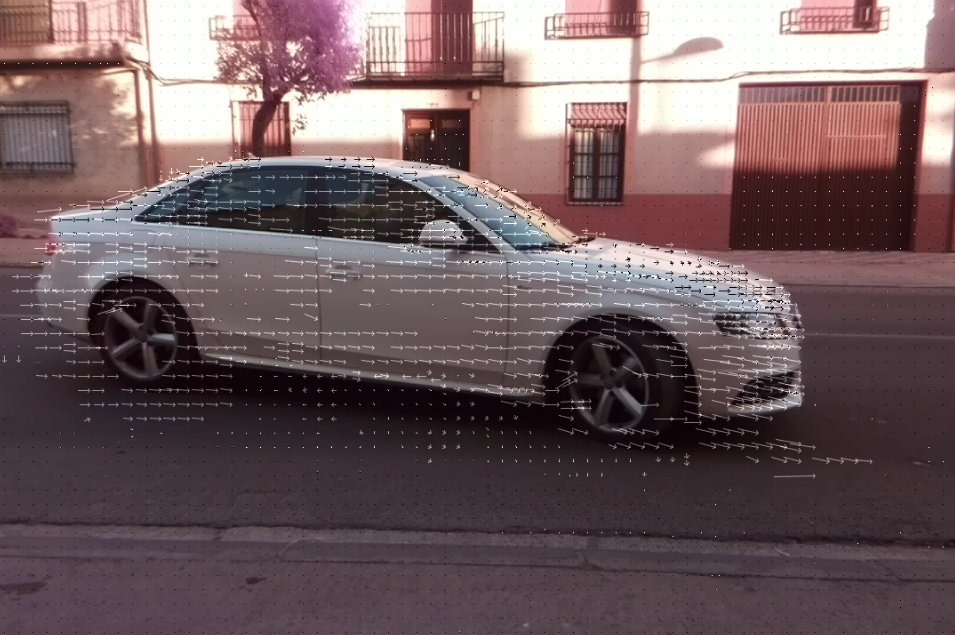
\includegraphics[width=0.8\textwidth]{6-Car_with_MV.png}
		\caption{Example of  the motion vectors taken by the Raspberry Pi}
		\label{fig:6-Car_with_MV}
	\end{center}
\end{figure}

The class used for recording the videos and the motion vectors used for developing the algorithm to count cars can be shown in Listing \ref{lst:6-Recorder-Sprint1}. Some parameters are given as arguments: \texttt{distance} and \texttt{angle}. They are used only for the filename so as to know afterwards the conditions of the camera when the video was recorded. In this class, the camera is configured according to the values stored in \texttt{config.py}. When the video has been recorded, it will be stored in a file with extension \texttt{.h264}, as well as the motion data, that will be stored in a file with the same name and extension \texttt{.data}. To finish with, the video will be also converted to \texttt{.mp4} to make easier its view in the development computer. 

\REDNOTE{IMPORTANT NOTE: Image resizer is not used. An other option is configure the camera resolution to 1920x1080 and use a resizer in the video to reduce the resolution given to the H.264 video coder.}

\lstinputlisting[language=Python, firstline=1, texcl, caption = {Class used to record a video and its corresponding motion data}, label = lst:6-Recorder-Sprint1]{code/6-Recorder-Sprint1.py}

\subsubsection{Develop a noise filter using moving averages}
There are some factors that can affect the number of motion vectors in a certain frame. Some of these factors can be the incorrect codification of that frame or a small object crossing the image (e.g., a person or a bug). Moreover, when H.264 video coding is used, there are several types of frame: I-frames, P-frames and B-frames \REDNOTE{(reference to their explanation)}. I-frames do not require other video frames to be decoded, therefore, they do not generate any motion vectors. Thus, the number of motion vectors in some frames is not going to be close to the reality, causing noise. To solve this problem, a smoothing technique is used. More concretely, simple moving averages calculation is applied.

A simple moving average \cite{Smi15} is a unweighted average of k prior values. Since a time series can be regarded as a sequence of values, $\{\overline {x_{t}}\}$, being $t=1,2,3,4,…n$, the moving average of these values can be computed. If we assume that $n$ is quite large, and we select an integer $k$ which is much smaller than $n$, we can compute the simple moving averages (of order k) as shown in Equation (\ref{eq:simple_moving_averages}).

\begin{equation} \label{eq:simple_moving_averages}
\overline { { x }_{ t } } =\frac { 1 }{ k } \sum _{ i=t-k+1 }^{ t }{ { x }_{ i } } ,\quad 2\le k\le n
\end{equation}

The result of applying the simple moving average over the data recorded previously can be shown in Figure \ref{fig:6-moving_averages}. Here, it can be appreciate how the graphic corresponding with the data before applying simple moving averages (black line) has some noise and sometimes it falls to 0. Additionally, it can be shown how the problem is decreased using this smoothing technique.

\begin{figure}[!h]
	\begin{center}
		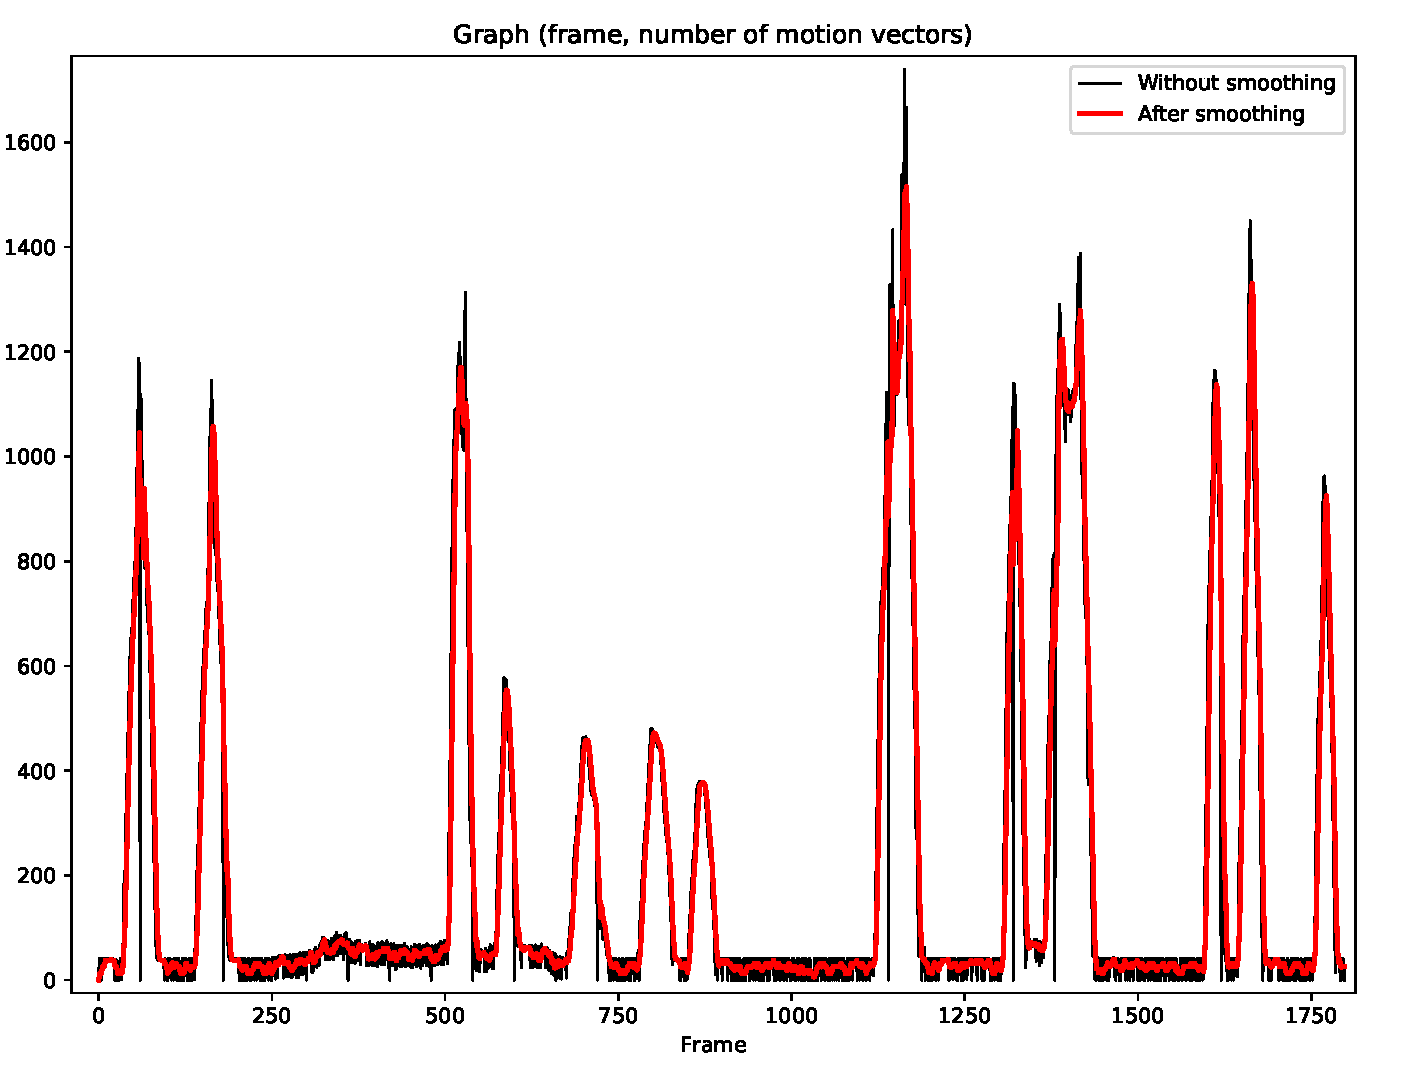
\includegraphics[width=1\textwidth]{6-moving_averages.pdf}
		\caption{Result of applying moving averages of order $n = 6$ to smooth the data}
		\label{fig:6-moving_averages}
	\end{center}
\end{figure}


\subsubsection{Develop the basic algorithm to counts the cars}
To count the cars that go across a street depending on its direction and using the motion data previously stored, an algorithm has been developed. Its pseudocode is shown in Algorithm \ref{alg:count_cars_V1}. This algorithm discriminates the cars direction (left or right). For each of the directions, the following algorithm is executed: 

For each frame, the number of motion vectors in that frame is compared with the number of vectors in the previous frame, increasing or decreasing a variable called \texttt{growth}. Once the number of frames exceed the \texttt{HEIGHT\_THRESHOLD} variable, if the \texttt{growth} variable is positive, the variable \texttt{n\_positive\_frames} is increased by one. If this last variable overtakes the \texttt{WIDTH\_THRESHOLD} variable, then it can be considererd that a new car has been detected. If the \texttt{growth} variable gets equal to \texttt{-GROWTH\_LIMIT}, then it is considered that the car has already passed, and the variable \texttt{n\_positive\_frames} is restored to its initial value (zero).

An example of the execution fo the algorithm can be shown in Figure \ref{fig:6-Count_cars_graphic}, where the blue line represents the number of motion vectors with left direction for each frame, and the red line represents the same but for right direction. The black line, represent the \texttt{HEIGHT\_THRESHOLD} variable. Therefore, a car can be predicted if the number of frames in one direction overtakes the \texttt{HEIGHT\_THRESHOLD} variable during more than \texttt{WIDTH\_THRESHOLD} frames. And, it can be considered that the car has already cross if the number of frames has been decreasing $\texttt{GROWTH\_LIMIT} \times 2 $ frames, regardless if the number of motion vectors is under the \texttt{HEIGHT\_THRESHOLD} variable or not. Therefore, in Figure \ref{fig:6-Count_cars_graphic}, it can be considered that two different cars have cross near the frame 1000, as the number of motion vectors has decreased during more than $\texttt{GROWTH\_LIMIT} \times 2 $ frames.

%\IncMargin{1em}
\begin{algorithm}
	\SetKwInOut{Input}{Input}\SetKwInOut{Output}{Output}
	\LinesNumbered
	\SetAlgoLined
	
	\Input{cols --> Number of colums with a macroblock in each frame\\
		rows --> Number of rows with a macroblock in each frame\\
		frames --> The number of frames in the video. \\
		motion\_data --> Array that contains a structure [x,y,SAD] for each frame} 
	\Output{n\_cars  --> Vector which contains the number of cars that has been counted crossing in left and right direction respectively.}
	
	n\_cars $\gets$ [0, 0]\;
	mv $\gets$ []\;
	smooth\_mv $\gets$ []\;
	car\_detected $\gets$ [False, False]\;
	growth $\gets$ [0, 0]\;
	n\_positive\_frames $\gets$ [0, 0]\;
	
	
	\For{frame $\gets$ 0 to frames}{
		%Add to the end of $mv$ vector a list with two elements. The first element consist in the number of motion vectors in that frame whose 'x' value is greather than the variable $GROUP\_SENSITIVITY$. The second element is the number of them whose 'x' value is lower than $-GROUP\_SENSITIVITY$.
		\tcc{Obtain number of motion vectors in each direction.}
		mv.append([ (motion\_data[frame]['x'] > GROUP\_SENSITIVITY).sum() ,
		(motion\_data[frame]['x'] < -GROUP\_SENSITIVITY).sum() ])\;
		
		\BlankLine
		\tcc{Apply moving averages to smooth the number of motion vectors}
		tmp\_left $\gets$ 0, tmp\_right $\gets$ 0\;
		\For{i $\gets$ 0 to SMOOT\_ORDER}{
			j $\gets$ frame - i\;
			\lIf{j < 0}{j $\gets$ 0}
			tmp\_left $\gets$ tmp\_left + mv[j][0] \;
			tmp\_right $\gets$ tmp\_right + mv[j][1]\;
		}
		smooth\_mv.append([tmp\_left / SMOOT\_ORDER, tmp\_right / SMOOT\_ORDER])\;
		
		\BlankLine
		\BlankLine
		\For{direction $\gets$ 0 to 2}{
			\uIf{smooth\_mv[frame-1][direction] < smooth\_mv[frame][direction]\\
				\hskip2em \textbf{and} growth[direction] < GROWTH\_LIMIT}{
				growth[direction] $\gets$ growth[direction] + 1\;
			}
			\ElseIf{smooth\_mv[frame-1][direction] < smooth\_mv[frame][direction]\\
				\hskip2em \textbf{and} growth[direction] > -GROWTH\_LIMIT}{
				growth[direction] $\gets$ growth[direction] - 1\;
			}
			
			\uIf{smooth\_mv[frame][direction] >= HEIGHT\_THRESHOLD \\
				\hskip2em \textbf{and} growth[direction] > 0}{
				n\_positive\_frames[direction] $\gets$ n\_positive\_frames[direction] + 1\;
				\If{n\_positive\_frames[direction] >= WIDTH\_THRESHOLD \\
					\hskip2em \textbf{and} car\_detected[direction] = False}{
					car\_detected[direction] $\gets$ True\;
					n\_cars[direction] $\gets$ n\_cars[direction] + 1\;
				}
				
			}
			\ElseIf{growth[direction] = -GROWTH\_LIMIT}{
				car\_detected[direction] $\gets$ False\;
				n\_positive\_frames[direction] $\gets$ 0\;
			}	
		}	
	}
	\caption{Count cars (First Version)}\label{alg:count_cars_V1}
\end{algorithm}\DecMargin{1em}

\begin{figure}[!h]
	\begin{center}
		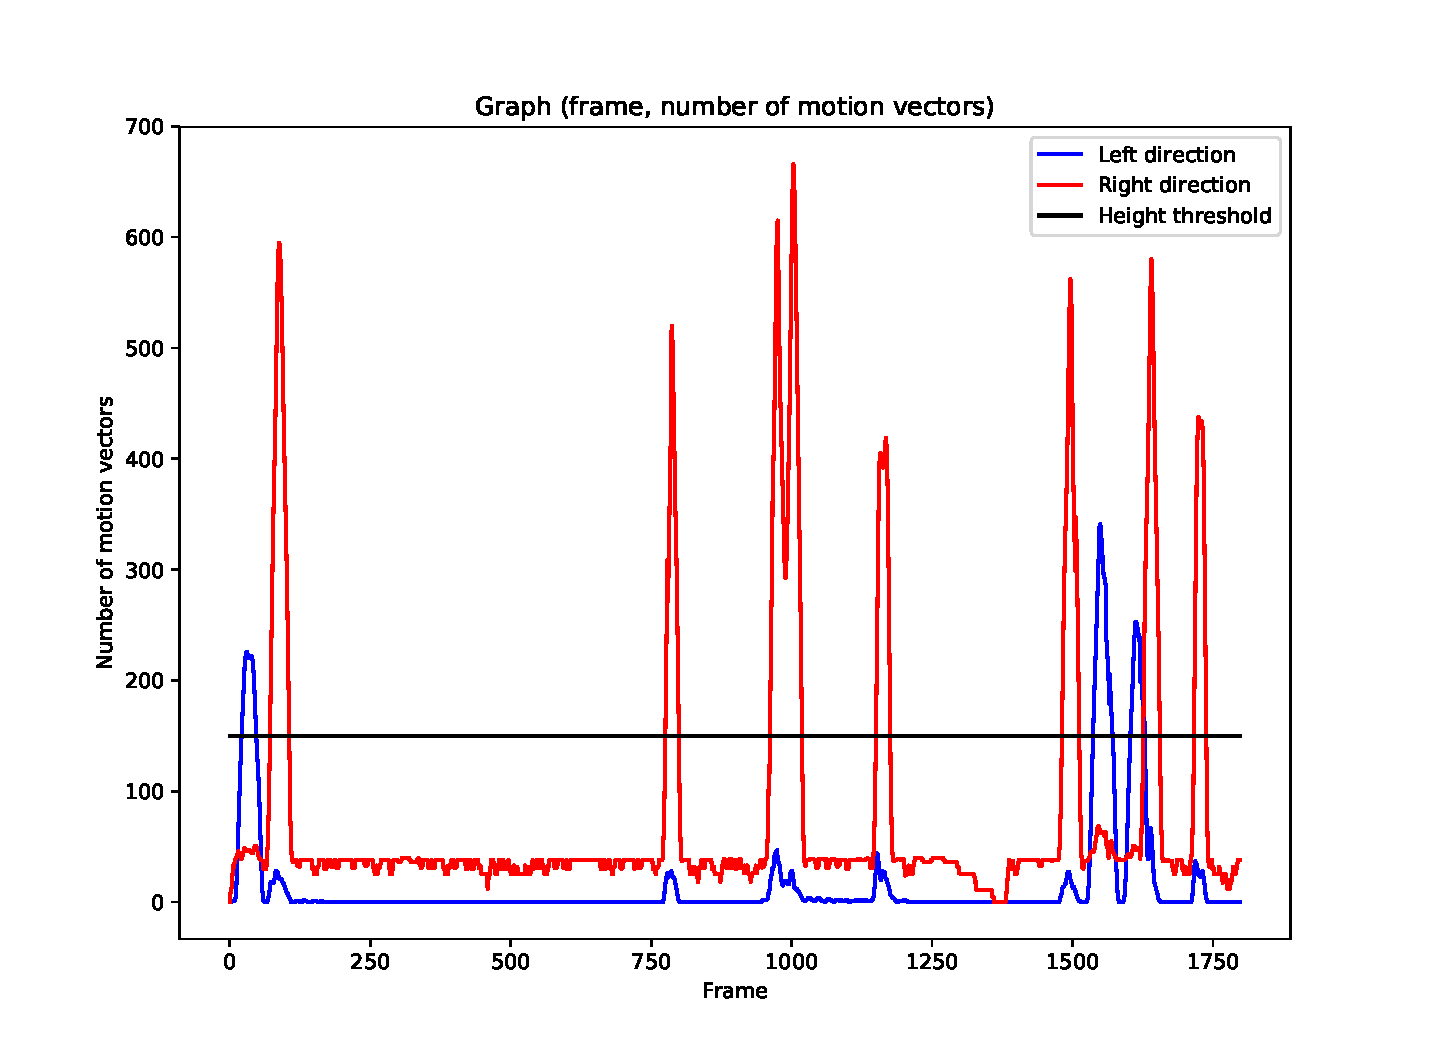
\includegraphics[width=1\textwidth]{6-Count_cars_graphic.pdf}
		\caption{Number of motion vectors in the test video 8}
		\label{fig:6-Count_cars_graphic}
	\end{center}
\end{figure}

Once the algorithm has been developed, it should be tested using the different videos recorded previously as it was stated in the list of test for the user story. The result of executing the algorithm over the different videos is shown in Table \ref{tab:Results_CountCars_V1}. After evaluating the results obtained, it is concluded that they are acceptable for the goal of this Sprint, therefore, a new Sprint can be started.

\begin{table}[hp]
	\centering
	{\small
		\begin{tabular}{ |P{.08\textwidth}P{.15\textwidth}P{.15\textwidth}P{.2\textwidth}P{.15\textwidth}|}
	\hline
	\rowcolor{tabheadbg}
	\multicolumn{5}{|c|}{\textscale{.8}{\textbf{Algorithm \ref{alg:count_cars_V1} results}}} \\
	\hline
	\hline
	\textscale{.8}{\textbf{Number}} & \textscale{.8}{\textbf{Quality}} & \textscale{.8}{\textbf{Camera angle}} & \textscale{.8}{\textbf{Distance to the road}} & \textscale{.8}{\textbf{Percentage of hits}} \\
	\hline
	1 	& 1080x720		 	&  center 		& 1m	& \textbf{100\%} \\ 
	\hline
	2 	& 1080x720		 	&  center 		& 1m	& \textbf{100\%} \\ 
	\hline
	3 	& 1080x720		 	&  center 		& 1m	& \textbf{90\%} \\ 
	\hline
	4 	& 1080x720		 	&  center 		& 2m	& \textbf{90.91\%} \\ 
	\hline
	5 	& 1080x720		 	&  center 		& 2m	& \textbf{100\%} \\ 
	\hline
	6 	& 1080x720		 	&  center 		& 2m	& \textbf{100\%} \\ 
	\hline
	7 	& 1080x720		 	&  center 		& 2m	& \textbf{94.74\%} \\ 
	\hline
	8 	& 1080x720		 	&  center 		& 3m	& \textbf{100\%} \\ 
	\hline
	9 	& 1080x720		 	&  center 		& 3m	& \textbf{90.91\%} \\ 
	\hline
	10 	& 1080x720		 	&  left 		& 1m	& \textbf{86.67\%} \\ 
	\hline
	11	& 1080x720		 	&  left 		& 1m	& \textbf{100\%} \\ 
	\hline
	12 	& 1080x720		 	&  left 		& 1m	& \textbf{100\%} \\ 
	\hline
	13 	& 1080x720		 	&  left 		& 2m	& \textbf{100\%} \\ 
	\hline
	14 	& 1080x720		 	&  left 		& 2m	& \textbf{55.56\%} \\ 
	\hline
	15 	& 1080x720		 	&  left 		& 2m	& \textbf{73.33\%} \\ 
	\hline
	16 	& 1080x720		 	&  left 		& 2m	& \textbf{88.89\%} \\ 
	\hline
	17 	& 1080x720		 	&  right 		& 1m	& \textbf{66.67\%} \\ 
	\hline
	18 	& 1080x720		 	&  right 		& 1m	& \textbf{78.57\%} \\ 
	\hline
	19 	& 1080x720		 	&  right 		& 1m	& \textbf{90\%} \\ 
	\hline
	20 	& 1080x720		 	&  right 		& 2m	& \textbf{83.33\%} \\ 
	\hline
	21 	& 1080x720		 	&  right 		& 2m	& \textbf{91.67\%} \\ 
	\hline
	22 	& 1080x720		 	&  right 		& 2m	& \textbf{88.89\%} \\ 
	\hline
	23 	& 1080x720		 	&  right 		& 2m	& \textbf{90\%} \\ 
	\hline
	\hline
	\multicolumn{3}{|c|}{\textscale{.8}{\textbf{Total number of tests: }} 23} & \multicolumn{2}{|c|}{\textscale{.8}{\textbf{Global percentage of hits: }} \textbf{89.57\%}} \\
	\hline
	
\end{tabular}
	}
	\caption{Results of the Algorithm \ref{alg:count_cars_V1} over the first test dataset}
	\label{tab:Results_CountCars_V1}
\end{table}


\REDNOTE{Task: Create a module that use the counting algorithm to obtain the vehicle flow in real time (using PiMotionAnalysis) in this Sprint or in another one.}



%%% Sprint 2
\section{Sprint 2: Design of an environmental parameters monitoring system}
In this Sprint, a program to obtain environmental data is going to be developed. This involves the implementation of some environmental sensors to measure some parameters such as temperature, humidity and pressure, as well as, the design and implementation of an electronic circuit to measure some contaminant gases. These gas sensors are going to be MQ-7 and MQ-2 sensors, which measures CO and LPG gases respectively. Once the circuit has been implemented, some code must be developed in order to control the sensors, as well as get the data they generate and store it into a data structure.

\subsection{Sprint planning meeting}
During the planning meeting, the two user stories addressed in this sprint has been analysed. These user stories are shown in Tables \ref{tab:Sprint2-User-story-4} and \ref{tab:Sprint2-User-story-5}.

\UserStoryTable{4}{2}{High}{25}
{Install environmental and gas sensors into Raspberry Pi}
{Design and implement the electronic circuit to integrate the different sensors into Raspberry Pi device.}
{	\item Install Raspberry Pi Sense Hat board
	\item Design an electronic circuit for the MQ gas sensors
	\item Connect the electronic circuit to Raspberry Pi device
}{	\item Check if the sensors are working correctly
	\item Test the connectivity of the Raspberry Pi with the external electronic circuit
}

\UserStoryTable{5}{2}{High}{30}
{Obtain and process data from the sensors}
{Develop a module that allows to communicate with the installed sensors and obtain the data.}
{	\item Develop a class that communicates with the external sensors using \ac{SPI}
	\item Develop a method to convert from the read values of the MQ sensors to particles per million
	\item Calibrate the MQ sensors
	\item Develop a method to control the different sensors and collect all the data
}{	\item Test the environmental sensors
	\item Test the MQ gas sensor
}

%Table \ref{tab:Sprint2-User-story-4}

\subsection{Results of the development of the tasks}

\subsubsection{Install Raspberry Pi Sense Hat board}
The installation of this board is very simple, as the only step is to place it correctly on top of the Raspberry Pi, making sure that the GPIO pins (Figure \ref{fig:6-Raspberry-Pinout-En}) are correctly aligned before pressing down firmly so the board properly attaches to the Raspberry Pi.

\subsubsection{Design an electronic circuit for the MQ gas sensors}
Due to the necessity of measuring some gases such as CO or Liquefied Petroleum Gas (LPG), some external sensors are needed, which are MQ-7 and MQ-2 sensors respectively. The MQ sensors are inexpensive gas sensors that are sensitive for a range of gasses and are recommended especially for indoor use. As we only want to obtain an approximate value of the polluting gases concentration (because accurate sensors are very expensive and require complex calibration methods), it has been decided to use these inexpensive sensors. Moreover, these sensors are quite common, so they can be obtained in lot of specialized stores. They provide an analogue signal output, hence a conversion to a digital value must be carried out. For this purpose an \ac{ADC} is needed, therefore the MCP3008 chip has been used \cite{MCP3008}.

As a result of the complexity of incorporating the MQ sensor directly to the electronic circuit, a chip module, which is shown in Figure \ref{fig:6-MQ_Sensor}, has been used instead. This chip implements the connections to the MQ sensor and provide 4 external connections (voltage, ground, digital output and analogue output). The digital output is not going to be used, as it only provides a logical value (1 or 0) according to a gas concentration threshold. Therefore, the analogue output is used and the value is converted to a digital one using the \ac{ADC} chip.

\begin{figure}[!h]
	\begin{center}
		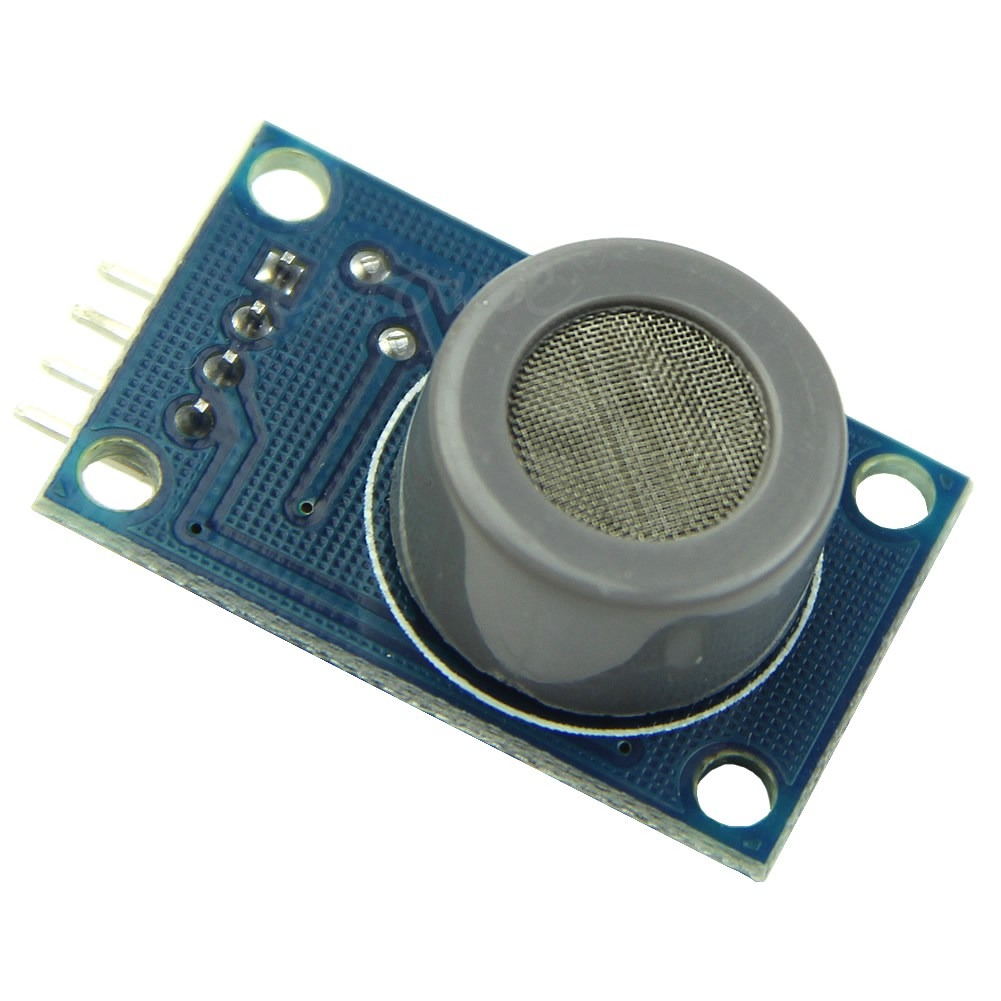
\includegraphics[width=0.5\textwidth]{6-MQ_Sensor.jpg}
		\caption{MQ sensor chip used}
		\label{fig:6-MQ_Sensor}
	\end{center}
\end{figure}

The implementation of the MQ-2 sensor is quite straightforward, however, the MQ-7 sensor require more attention. This is because MQ-7 sensor works in cycles of two phases: First the sensor is powered by 1.4 volts during 60 seconds. At the end of this phase, the results are read from the sensor and then a phase of 90 seconds starts where the sensor is heated with 5 volts (which allows the sensor to clean up for the next measurement). In the case of the MQ-2 sensor, the 5 volts which are necessary in order to power it can be supplied by the 5 volts power supply (Pin 4) of the GPIO interface as shown in Figure \ref{fig:6-Raspberry-Pinout-En}, which can supply up to 700 mA. In the case of the MQ-7 sensor, \ac{PWM} is going to be used to generate the 1.4 volts, but the GPIO pins used for the \ac{PWM} can only supply 50 mA. This sensor consume approximately 150 mA and therefore the Raspberry pin can burn. To solve this problem the LM317 chip has been used, which is a regulator capable of supplying more than 1.5 Amperes over an output-voltage range of 1.25 volts to 37 volts \cite{LM317}. By using LM317 chip, the current is drawn form the 5 volts power supply and the pin BCM 16 can be used without any problem for generating a \ac{PWM}.

\ac{PWM} is a modulation technique that allow generating waveforms of high frequencies and high precision \cite{DdlT16}, and it can be used to control the power supplied to electrical devices, such as motors. To generate a \ac{PWM} signal it is needed to define the period and the duty cycle (Figure \ref{fig:6-PWM-signal}). The period indicates duration of each cycle, whereas the duty cycle describes the proportion of the period in which the signal is in high power state (in this case 3.3 volts, which is voltage generated by the GPIO pins). The frequency (which is the inverse of the period) has been defined to $100 Hz$ which is enough, and taking this value into account the duty cycle has been defined to $14\%$ in order to obtain 1.4 volts and to $100\%$ to obtain the maximum voltage allowed by the LM317 chip (for the heating phase). The final circuit is shown in Figure \ref{fig:6-Circuit-Schematic}.

\begin{figure}[!h]
	\begin{center}
		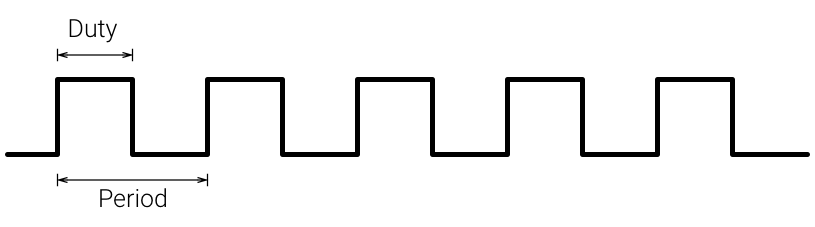
\includegraphics[width=0.75\textwidth]{6-PWM-signal.png}
		\caption{PWM signal}
		\label{fig:6-PWM-signal}
	\end{center}
\end{figure}

The consequence of using the LM317 chip is that it has an internal drift that we have measured as approximately 1.8 volts and, consequently, only 3.2 volts can be generated using a 5 volts power supply. Since the 5 volts phase is only used to heat the sensor, there is not a big difference in the precision of the measurements, hence this solution is going to be accepted for this prototype. In a final implementation, two solutions can be implemented to solve this problem. The first one is to use a higher voltage power supply (which is a simple solution if the device is connected to the street lighting power supply). A second approach consist in implement a circuit using transistors to switch between 1.4 and 5 volts. This second solution has not been implemented as it exceeds the objectives of this \ac{BSc.} thesis.


% https://easyeda.com/editor
\begin{figure}[!h]
	\begin{center}
		\includegraphics[width=1\textwidth]{6-Circuit-Schematic.pdf}
		\caption{Circuit schematic}
		\label{fig:6-Circuit-Schematic}
	\end{center}
\end{figure}

\begin{figure}[htb]
	\centering
	\subfigure[Raspberry Pi Pinout Board Schema]{
		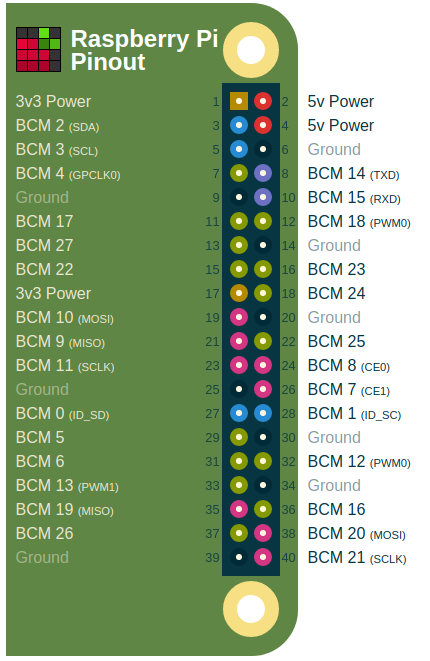
\includegraphics[height=0.82\textwidth,angle=90]{6-Raspberry-Pinout-En.png}
		\label{fig:6-Raspberry-Pinout-En}
	}
	\subfigure[Raspberry Pi Pinout Connections]{
		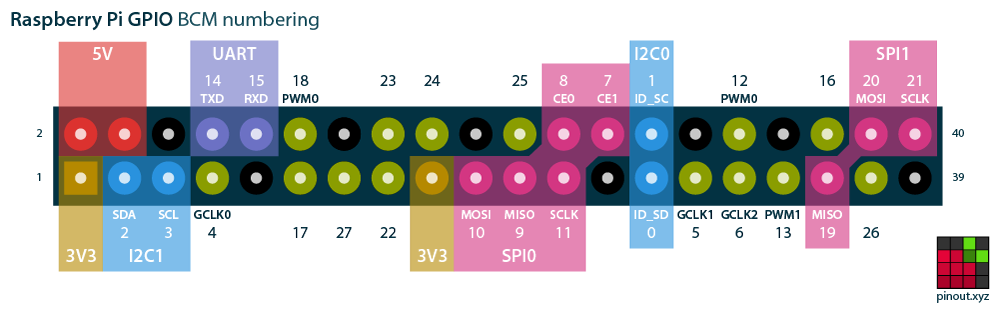
\includegraphics[width=1\textwidth]{6-Raspberry-Pinout-Expanded.png}
		\label{fig:6-Raspberry-Pinout-Expanded}
	}
	\caption{Raspberry Pi Pinout}
	\label{fig:6-Raspberry-Pinout}{Source: \url{https://pinout.xyz/}}
\end{figure}




\subsubsection{Connect the electronic circuit to Raspberry Pi device}
The next step is to connect the previous electronic circuit to the Raspberry Pi. For this purpose the GPIO pins are going to be used. However, as the Sense hat module has been installed in the Raspberry Pi, not all the GPIO pins are available. These pins can be located in Figure \ref{fig:6-Raspberry-Pinout-Expanded} or using the webpage \url{https://pinout.xyz/} where all the information about the different pins is displayed. Therefore, for the \ac{SPI} communication with the MCP3008 chip the pins BCM  18, 19, 20, and 21 are used. In addition, pin BCM 16 is used for \ac{PWM} and GPIO 4 and 6 for 5 volts power and ground respectively. Figure \ref{fig:6-Electric_diagram.pdf} shows the connection diagram of the components using a protoboard to connect them.

\begin{figure}[!h]
	\begin{center}
		\includegraphics[height=1\textwidth,angle=90]{6-Electric_diagram-cropped.pdf}
		\caption{Connection diagram of the components}{Image generated using fritzing}
		\label{fig:6-Electric_diagram.pdf}
	\end{center}
\end{figure}


\subsubsection{Develop a class that communicates with the external sensors using \ac{SPI}}
As it has been previously commented, the analogue output from the MQ sensors will be converted to a digital value using an \ac{ADC} chip. For this purpose, the MCP3008 chip \cite{ADC} is going to be used, which communicates with the processor using \ac{SPI} protocol. The class developed need to implement this protocol internally in order to obtain the data form this chip using the GPIO pins (Listing \ref{lst:6-spiCommunicator}). The protocol has been implemented following the specifications of the MCP3008 datasheet (Figure \ref{fig:6-MCP3008-SPI}), where all the signals that need to be activated in each clock cycle are stated. The channel is going to be provided as argument, being channel 0 the MQ-7 sensor and channel 1 the MQ-2 sensor, as it was stated in the wiring connections of Figure \ref{fig:6-Circuit-Schematic}.

\begin{figure}[!h]
	\begin{center}
		\includegraphics[width=0.9\textwidth]{6-MCP3008-SPI.pdf}
		\caption{Communication with SCP3008}{Image from MCP3008 datasheet \cite{ADC}}
		\label{fig:6-MCP3008-SPI}
	\end{center}
\end{figure}

\lstinputlisting[language=Python, firstline=27, texcl, caption = {\emph{read} method from \texttt{spiCommunicator.py} file}, label = lst:6-spiCommunicator]{code/6-spiCommunicator.py}


\subsubsection{Develop a method to convert from the read values of the MQ sensors to particles per million}
The values provided by the previous class corresponds to the voltage of the current that goes through the sensor and it need to be converted to particles per million of the gas measured. For this purpose the sensitivity characteristic curve of the different gases (Figure \ref{fig:6-MQ_curve}) defined in the sensor documentation must be studied. This curve explains how the resistance of the sensor changes depending on the concentration of the target gas. Therefore, the first step must be calculating the resistance of the sensors. 

The value provided by the \ac{SPI} protocol need to be converted in order to obtain the real value of the voltage. In the MCP3008 chip documentation \cite{ADC} the Equation \ref{eq:digital_output_code_calculaiton} is purposed to calculate the value given by the converter ($adc$), where ${V}_{RL}$ is the value of the voltage being measured in the corresponding channel of the converter and ${V}_{R}$ the reference level used by the converter.
\begin{equation} \label{eq:digital_output_code_calculaiton}
adc = \frac { 1024\cdot { V }_{ RL } }{ { V }_{ R } } 
\end{equation}
This equation can be modified to obtain the real value of the voltage going through the gas sensor, as shown in Equation \ref{eq:VRL}.
\begin{equation} \label{eq:VRL}
{ V }_{ RL } =\frac { adc \cdot  { V }_{ R }}{ 1024 }  
\end{equation}

The reference level used by the \ac{ADC} chip is going to be the same as the used for the rest of the circuit (5 Volts), as shown in Equation \ref{eq:ref_voltage}.
\begin{equation} \label{eq:ref_voltage}
{V}_{R} = {V}_{C}
\end{equation}

To obtain the resistance of the MQ sensors, their official documentation \cite{MQ7,MQ2} purpose the use of the Equation \ref{eq:operational_principle}, where ${R}_{S}$ is the current resistance of the sensor (in $K\Omega$, i.e. 1000 ohms), ${R}_{L}$ is the load resistance in $K\Omega$ (i.e. the external resistance connected to the sensor) and ${V}_{RL}$ is the value of the voltage being measured. 
\begin{equation} \label{eq:operational_principle}
{ { R }_{ S } }/{ { R }_{ L } }=\frac { { V }_{ C }-V_{ RL } }{ V_{ RL } } 
\end{equation}

Combining Equations \ref{eq:VRL}, \ref{eq:ref_voltage} and \ref{eq:operational_principle}, the final Equation \ref{eq:Rs_equation} is obtained, which allows us to calculate the value of the MQ gas sensor resistance using the raw value obtained by the \ac{ADC} chip (denoted as $adc$).
\begin{equation} \label{eq:Rs_equation}
\begin{aligned}
{ { R }_{ S } }/{ { R }_{ L } }=\frac { { V }_{ C }-V_{ RL } }{ V_{ RL } } \Rightarrow 
{ { R }_{ S } }/{ { R }_{ L } }=\frac { { V }_{ C }-\frac { adc\cdot { V }_{ C } }{ 1024 }  }{ \frac { adc\cdot { V }_{ C } }{ 1024 }  } \Rightarrow \\
{ { R }_{ S } }/{ { R }_{ L } }=\frac { 1024\cdot { V }_{ C }-adc\cdot { V }_{ C } }{ adc\cdot { V }_{ C } } \Rightarrow 
{ R }_{ S }=\frac {  { R }_{ L } \cdot (1024-adc) }{ adc } 
\end{aligned}
\end{equation}

Listing \ref{lst:6-getResistance} shows the implementation of the previous equation into python code.
\lstinputlisting[language=Python, firstline=1, texcl, caption = {\emph{getResistance} method from \texttt{Sensors.py} file}, label = lst:6-getResistance]{code/6-getResistance.py}

To avoid outliers caused by some incorrect measurements, the final value of the resistance will be taken as the mean value of \texttt{READ\_SAMPLE\_TIMES} samples taken each \texttt{READ\_SAMPLE\_INTERVAL} milliseconds at shown in Listing \ref{lst:6-Read}.

Once the value of the MQ sensor resistance is known, the second step will be to convert it to particles per million (ppm). In order to achieve it, the corresponding MQ characteristic curve defined in its documentation must be implemented. For the purposes of simplicity, instead of defining the logarithm curved defined in the documentation, base ten logarithms will be taken in order to obtain a straight line and simplify the calculations, as it is shown in Figure \ref{fig:6-MQ_curve}. The abscissa axis represent the ppm concentration of the target gas, whereas the ordinate axis represent the ${R}_{S}/{R}_{O}$ quotient, where ${R}_{S}$ is the resistance of the sensor calculated in Equation \ref{eq:Rs_equation} and ${R}_{O}$ is the resistance of the sensor (calculated with the same equation) at a certain concentration of the gas that depends on the sensor. This ${R}_{O}$ parameter need to be adjusted for every sensor, as it is used to calibrate the measurements.

\begin{figure}[htb]
	\centering
	\subfigure[MQ-7]{
		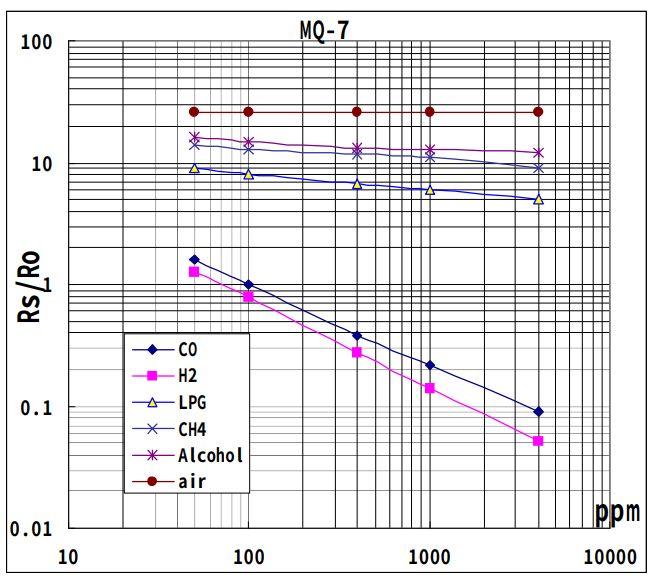
\includegraphics[width=0.48\textwidth]{6-MQ-7_curve.png}
		\label{fig:6-MQ-7_curve}
	}
	\subfigure[MQ-2]{
		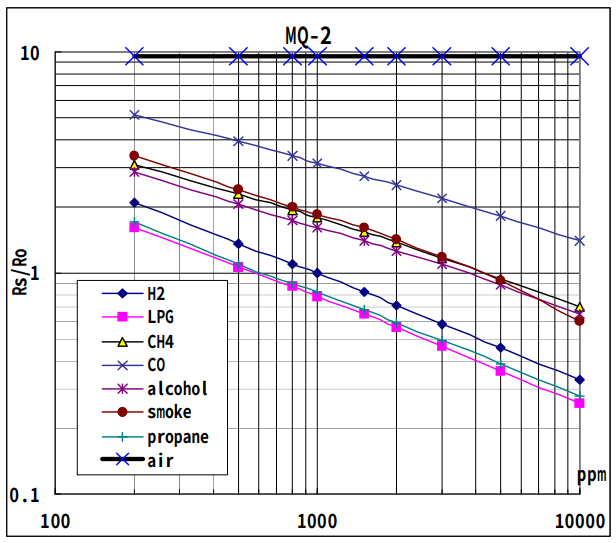
\includegraphics[width=0.48\textwidth]{6-MQ-2_curve.png}
		\label{fig:6-MQ-2_curve}
	}
	\caption{Sensitivity characteristic curve of the MQ sensors}
	\label{fig:6-MQ_curve}{Source: MQ sensor documentation \cite{MQ7,MQ2}}
\end{figure}

Therefore, to convert from the sensor resistance to ppm, the slope and the y-intercept of the line must be calculated for both sensors \cite{ConfMQX}. For example, to calculate the line that defines the CO concentration in the MQ-7 sensor, first, it is needed to calculate the slope of the line as shown in Equation \ref{eq:CO_slope}.
\begin{equation} \label{eq:CO_slope}
m=\frac { { y }_{ 2 }-{ y }_{ 1 } }{ { x }_{ 2 }-{ x }_{ 1 } } =\frac { \log _{ 10 }{ 0.09 } -\log _{ 10 }{ 1.8 }  }{ \log _{ 10 }{ 4000 } -\log _{ 10 }{ 50 }  } =-0.68
\end{equation}
The next step is to calculate the y-intercept of the line. Then, the left point of the line is taken and the base ten logarithm is applied, giving as a result the point $(x=1.7, y=0.26)$. These calculations must be repeated for the LPG measured by the MQ-2 sensor.

Now the line is calculated, the methods to convert from resistance to ppm can be developed as shown in Listing \ref{lst:6-getMQPPM}.

\lstinputlisting[language=Python, firstline=1, texcl, caption = {\emph{getMQPPM} method from \texttt{Sensors.py} file}, label = lst:6-getMQPPM]{code/6-getMQPPM.py}

The last step is to develop a method to obtain the final value from the sensor given the channel where it is connected. This method is shown in Listing \ref{lst:6-Read}

\lstinputlisting[language=Python, firstline=1, texcl, caption = {\emph{read} method from \texttt{Sensors.py} file}, label = lst:6-Read]{code/6-Read.py}


\subsubsection{Calibrate the MQ sensors}
The MQ sensor documentation purpose as a calibration method to generate a certain concentration of a given gas and measure the resultant resistance of the sensor. For example, for MQ-7 sensor, a concentration of 100ppm of CO in clean air is needed. Nevertheless, we have not enough resources to generate this gas concentration, and other calibration methods have been studied, such as measuring the current concentration of the gas with another CO sensor and compare the results, but it was not possible either. 

Therefore, an alternative approach have been developed in order to obtain an approximate value for ${R}_{O}$. It consists in locating the sensor into clean air (with not or not much CO and LGP contamination) and then measure the sensor resistance (${R}_{S}$). Then, the sensitivity curve of clean air for the given sensor can be calculated and used to obtain ${R}_{O}$, as shown in lines 16-19 of Listing \ref{lst:6-MQCalibration}, where \texttt{MQ\textbf{X}\_RO\_CLEAN\_AIR\_FACTOR} is the value of the clean air on the ordinate axis for the sensor sensitivity characteristic curve (Figure \ref{fig:6-MQ_curve}). This calculation will be repeated a certain number of times in order to obtain more accurate values. These steps have to be repeated for all units installed of each sensor type (MQ-7 and MQ-2), as the values changes depending on every sensor.

\lstinputlisting[language=Python, firstline=1, texcl, caption = {\emph{calibration} method from \texttt{Sensors.py} file}, label = lst:6-MQCalibration]{code/6-MQCalibration.py}

With this approach an approximate value of the gas concentration can be obtained, which is enough for this \ac{BSc.} thesis. Nonetheless, in a real implementation the sensor must be correctly calibrated, in order to obtain the real gas concentration.


\subsubsection{Develop a method to control the different sensors and collect all the data}

In order to control and collect the data from all the previous sensors a new method have to be developed. Firstly, the necessary GPIO pins for the sensors are going to be configured, as well as the \ac{PWM} cycle for controlling the voltage of the MQ-7 sensor is going to be initialized. Secondly, all the sensor data form the MQ sensors and from the environment sensors installed in the Sense Hat \cite{SenseHAT} are going to be obtained.

In order to avoid noisy data or sudden changes on the data, a smoothed average is going to be applied as it is shown in Equation \ref{eq:smoothed_average}, where ${w}_{t+1}$ represents the actual data read by the sensor, $\overline{{w}_{t}}$ is the value calculated by the equation in the previous measure and $\alpha$ is a factor that indicates how much new values affect to the final value represented as $\overline{{w}_{t+1}}$.
\begin{equation} \label{eq:smoothed_average}
\overline { { w }_{ t+1 } } =\alpha \cdot { w }_{ t+1 }+(1-\alpha )\cdot \overline { { w }_{ t } } 
\end{equation}
The $\alpha$ coefficient must be calculated in order to make the influence of the $n^\text{th}$ previous measurement negligible. Therefore, Equation \ref{eq:epsilon} can be demonstrated from the previous one, where the maximum influence of the $n^\text{th}$ previous measurement ($\varepsilon$) is calculated.
\begin{equation} \label{eq:epsilon}
{ (1-\alpha ) }^{ n }<\varepsilon  
\end{equation}
If we suppose that $\varepsilon$ is negligible with a value of ${10}^{-3}$, and we only want that the last half hour has influence over the data taking the values from the sensors each 2.5 minutes, then $n$ must be 12. We can operate on the previous equation to obtain the Equation \ref{eq:gamma_value}.
\begin{equation} \label{eq:gamma_value}
{ (1-\alpha ) }^{ n }<\varepsilon \Rightarrow 1-\alpha <\sqrt [ n ]{ \varepsilon } \Rightarrow 1-\sqrt [ n ]{ \varepsilon }<\alpha
\end{equation}
Then, considering $n=12$ and $\varepsilon={10}^{-3}$, the value calculated is $\alpha=0.57$, which is the one that will be used.

These parameters are going to be used to adjust Equation \ref{eq:smoothed_average} obtaining the final equation. At this point, the Sprint has been completely finished and the Raspberry Pi device can obtain not only environmental and pollution information, but also the traffic flow as it was explained in section \ref{Section:Sprint1}.


%%% Sprint 3
\section{Sprint 3: Development a module to send data from Raspberry Pi to the cloud and store it into a Database}
\REDNOTE{...}
% Product Backlog refinement

\subsection{Sprint planning meeting}
\REDNOTE{...}

%\UserStoryTable{6}{3}{High}{x}
%{Name of the user story}
%{A description of the user story}
%{	\item Task A
%	\item Task B
%	\item Task C
%}{	\item Test A
%	\item Test B
%}

%Table \ref{tab:Sprint2-User-story-4}

\subsection{Results of the development of the tasks}
\textbf{task something ...}

\REDNOTE{...}


%%% Sprint 4
\section{Sprint 4: Development of a program to monitor the data in real time and control the Raspberry Pi systems}
\REDNOTE{...}
% Product Backlog refinement

\subsection{Sprint planning meeting}
\REDNOTE{...}

%\UserStoryTable{4}{3}{High}{x}
%{Name of the user story}
%{A description of the user story}
%{	\item Task A
%	\item Task B
%	\item Task C
%}{	\item Test A
%	\item Test B
%}

%Table \ref{tab:Sprint2-User-story-4}

\subsection{Results of the development of the tasks}
\textbf{task something ...}

\REDNOTE{...}



%%%% Sprint X
%\section{Sprint X: ....}
%\REDNOTE{...}
%% Product Backlog refinement
%
%\subsection{Sprint planning meeting}
%\REDNOTE{...}
%
%%\UserStoryTable{4}{3}{High}{x}
%%{Name of the user story}
%%{A description of the user story}
%%{	\item Task A
%%	\item Task B
%%	\item Task C
%%}{	\item Test A
%%	\item Test B
%%}
%
%%Table \ref{tab:Sprint2-User-story-4}
%
%\subsection{Results of the development of the tasks}
%\textbf{task something ...}
%
%\REDNOTE{...}
%
%\subsection{Daily Scrum}
%\REDNOTE{...}
%
%\subsection{Sprint review}
%\REDNOTE{...}
%
%\subsection{Sprint retrospective}
%\REDNOTE{...}
